\chapter{IMPLEMENTATION}\label{chap:IMPLEMENTATION}

\hspace{0.5in}This chapter describes how to implement the Face Replacement System. It includes system environments that describe the requirements of the Face Replacement System, the process of implementing a user interface, and also the Face Replacement System.

\section{System Environment}
Operating System and Utilities Application requirements
\begin{itemize}
\item Operating System
    \begin{itemize}
    \item Microsoft Windows with .NET Framework 3.5 SP1
    \end{itemize}
\item Integrated Development Environment
    \begin{itemize}
    \item Microsoft Visual Studio 2008
    \item Microsoft Expression Blend 3
    \end{itemize}
\item Additional Library
    \begin{itemize}
    \item OpenCV library with Emgu.CV-2.0.1.0 wrapper
    \item dnAnalytics 2009.8
    \end{itemize}
\end{itemize}


\section{Implementation of the User Interface}
\hspace{0.5in}Windows Presentation Foundation (WPF) is a next-generation presentation system for building Windows client applications. We use WPF in order to create the graphical user interface which looks more attractive and easy to use. The main functionality of our interface is the ability to drag and drop the items. For this interface, users can drag photograph files into the application window. The photo will show on the interface. The application will detect faces automatically and shows the  line of face contour. To do the face replacement, users drag a face to any other face they want. The replacement will be done automatically and the result will be shown when it finishes. Users can keep a face to use across photos by dragging a face into the box below. Later on, users can drag a face from the box to another face in a photo that the users want.

\begin{figure}[htb]
   \centering
   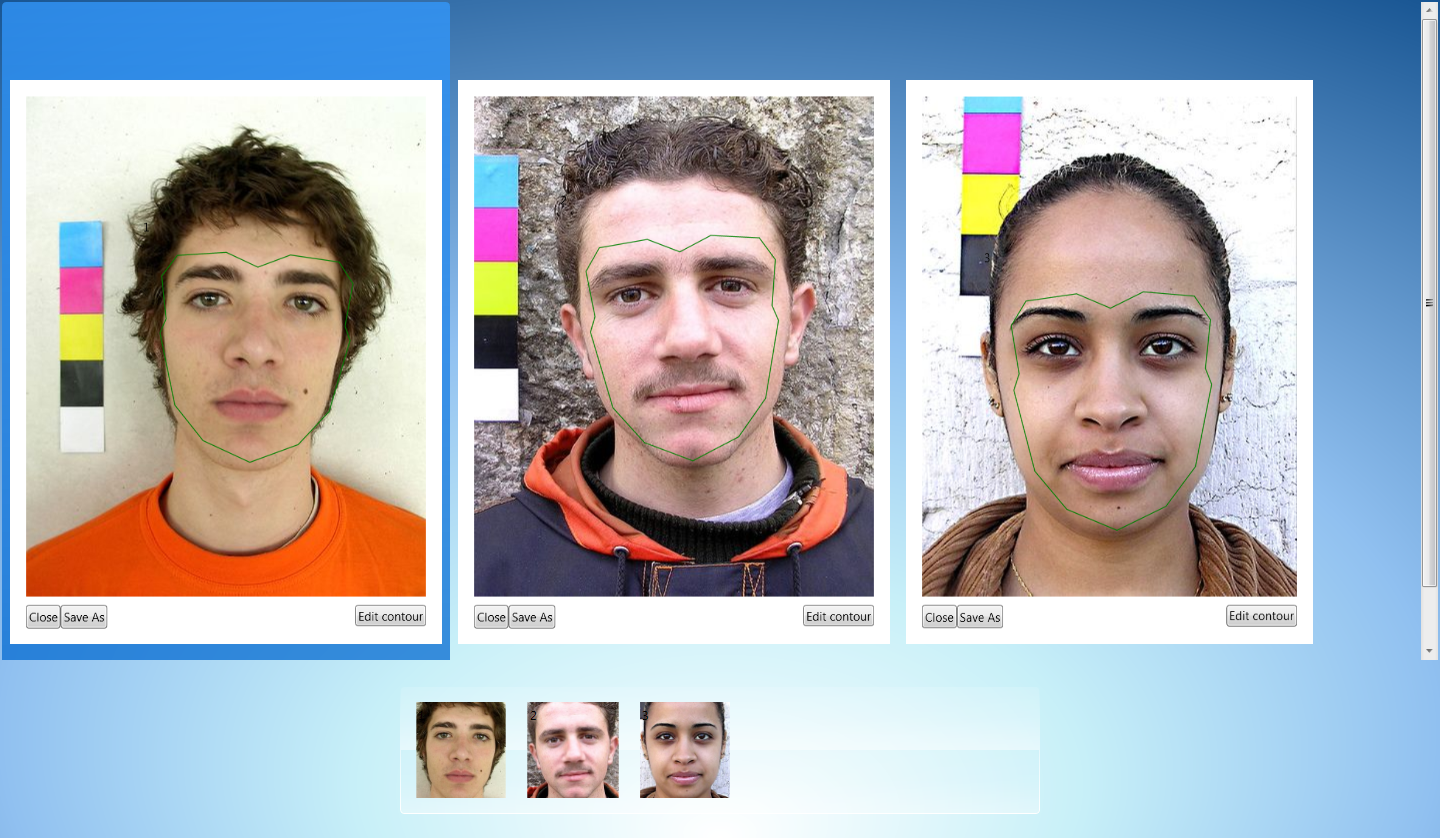
\includegraphics[width=15cm]{main.png}
   \caption{The Early Version of the User Interface of the Face Replacement System}
   \label{fig:InterfaceFace}
\end{figure}

Sometimes, the face detector fails to detect the precisely correct position, and results in an incorrect face contour. The edit button is available for editing the face contour manually by the users. Users can improve the correctness of the contour by adjusting the contour to cover only the facial skin and avoid having the contour cross any details.

\section{Implementation of the Face Replacement Engine}

\hspace{0.5in}We have implemented the Face Replacement System using C\# language because it is a high-level language and there is the unsafe code feature which allows some portion of code to be executed with low overhead as low-level language. It is also a current flagship language from Microsoft that can integrate with most Microsoft Technology such as WPF.

\begin{figure}[htb]
   \centering
   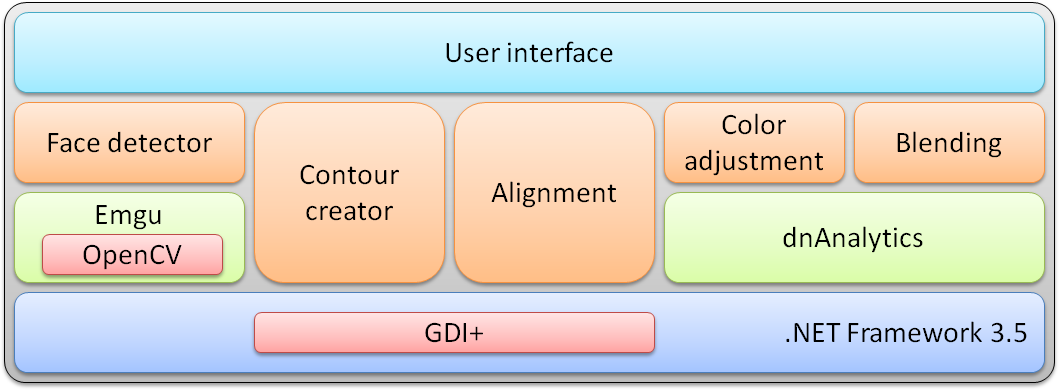
\includegraphics[width=13cm]{architecture.png}
   \caption{The Face Replacement System Architecture Diagram}
   \label{fig:ArchitectureDiagram}
\end{figure}

For the face detection part, we have developed the functionality of face detection from Emgu, which is the wrapper of OpenCV. There are cascade trained files used for detecting face, eyes, and mouth, which are published by Modesto Castrillon Santana \cite{website:ModestoCastrillonSantana}. We have implemented the face detection to be able to detect the face region. Then, we divide the subregions and use them to detect eyes and mouth. We divide the subregions to be top-left for left eye, top-right for right eye, and below for mouth. There is a high possibility that the eye detection will give a false positive result. We assume that if it detects more than one eye position at each side of eyes, we will choose the one which is the nearest to 30\% from each side.

As we did not use the commercial face detector as used in Bitouk's paper \cite{Bitouk2008}, which is able to detect the face with out-of-plane pose, we have considered only 2D plane poses.

For the face contour creation part, there are trigonometric functions available. There are Point and Vector classes which can be used for calculating the vector length and angle between vectors in a 2D plane.

We have developed a separate program for training a face contour. This program was written to help collect face contour training information. This program is not intended for end users because training face contours is not an end users' task. The face contour training program will be described in the section "Preparation of contour initiation data" later in this chapter.

For the alignment part, there is the Matrix class, which is used for transformation and is in the GDI+ library, which is wrapped in the .NET Framework, so we can define a set of operations such as rotate, translate, and scale. Then, we can use the matrix to transform the image and contour.

The color adjustment part has been implemented as suggested in the paper. We have also implemented our modified version which clones color distribution by percentiles from an image to another image.

For the blending part, there are two algorithms, Poisson and Mean-Value Coordinates. In the early stage of development, we have integrated the source code of the Poisson Image Editing, which is the open source project provided online by Tommer Leyvand \cite{website:TommerLeyvand}. The Poisson Image Editing source code is written in unmanaged C++ but our system was developed in .NET Framework environment. So, we have to study how it works and port the system from this source code in order to get the same functionality.

The contour obtained from the contour creation part will be used as loose selection input for Poisson cloning. Therefore, we have to render the contour to be mask area. We use GDI+ library to render this masking. As the original Poisson Image Editing source code is developed in C++, it uses TAUCS as a linear sparse matrix solver in order to solve the Poisson equation.

As we have implemented the system on the .NET platform, a problem occurs when we try to combine our system with old static library, which is an unmanaged code. So, we have to select another linear solver that can work with our system. We have selected dnAnalytics, which is an open source numerical library written in C\#, and also supports sparse matrix.

Another blending algorithm is Mean-Value Coordinates algorithm. In the later stage, we have developed this algorithm according to the research paper. dnAnalytics also contains statistics facilities so we use it in some steps of this calculation.

\section{Preparation of Contour Initiation Data}

\hspace{0.5in}We have developed a separate program for face contour training. The purpose of this program is to extract information regarding face contour, including the position of eyes and mouth, and sixteen contour points around a face, gathered from many faces to define contour initiation data. The program will collect raw data as absolute positions. This raw data will be converted to relative positions from main face features to face contour positions, be averaged to be a converged relationship, and then will be used as a predefined relationship to construct a face contour that can be approximately matched with any face.

The face images that we have used for training face contours are from the Face of Tomorrow collection by photographer Mike Mike on Flickr istanbulmike's photostream \cite{website:faceimages}. We have randomly selected 124 images which are approximately sized 400${\times}$500 pixels in order to do the face contour training.

The usage of this program is to record the feature positions from a large collection of face images. At first, trainers have to define the position of left eye, right eye, and mouth sequentially. Then, the 16 contour points will appear on the face image which might not exactly match to the face contour. What trainers have to do is to manually edit each contour point to be at the appropriate position as the face contour, and then save the contour points information into a file.

\begin{figure}[htb]
   \centering
   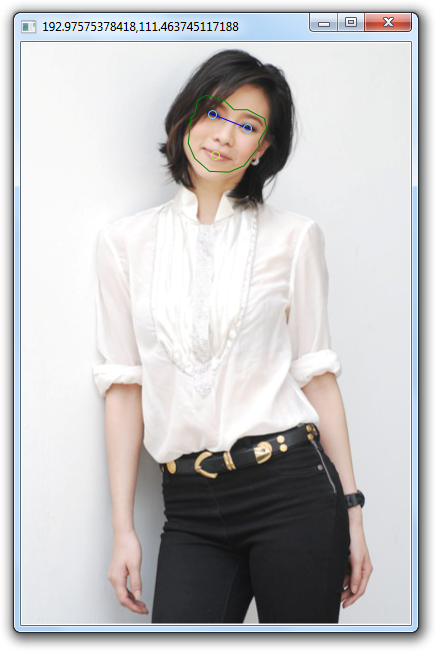
\includegraphics[width=4.5cm]{train.png}
   \caption{The Face Contour Training Program}
   \label{fig:InterfaceTrain}
\end{figure} 